\documentclass[12pt]{article}
\usepackage[utf8]{inputenc}
\usepackage[english,russian]{babel}
\usepackage{a4wide}
\usepackage{graphicx}
\usepackage{amssymb}
\usepackage{amsmath}
\usepackage{color}
\usepackage{url}
\usepackage{tikz}
\usetikzlibrary{matrix}

\DeclareMathOperator*{\argmax}{arg\,max}
\DeclareMathOperator*{\argmin}{arg\,min}
\newcommand*{\No}{No.}

\usepackage[pdftex,unicode, 
colorlinks=true,
linkcolor = blue
]{hyperref}	% нумерование страниц, ссылки!!!!ИМЕННО В ТАКОМ ПОРЯДКЕ СО СЛЕДУЮЩИМ ПАКЕТОМ
\newcommand{\hdir}{.}
%\linespread{2} %Потом убрать
\newcommand{\bx}{\mathbf{x}}
\newcommand{\by}{\mathbf{y}}
\newcommand{\bw}{\mathbf{w}}
\newcommand{\ba}{\mathbf{a}}
\newcommand{\bz}{\mathbf{z}}
\newcommand{\bb}{\mathbf{b}}
\newcommand{\bY}{\mathbf{Y}}
\newcommand{\bX}{\mathbf{X}}
\newcommand{\bu}{\mathbf{u}}
\newcommand{\bt}{\mathbf{t}}
\newcommand{\bp}{\mathbf{p}}
\newcommand{\bq}{\mathbf{q}}
\newcommand{\bc}{\mathbf{c}}
\newcommand{\bP}{\mathbf{P}}
\newcommand{\bT}{\mathbf{T}}
\newcommand{\bB}{\mathbf{B}}
\newcommand{\bQ}{\mathbf{Q}}
\newcommand{\bC}{\mathbf{C}}
\newcommand{\bE}{\mathbf{E}}
\newcommand{\bF}{\mathbf{F}}
\newcommand{\bU}{\mathbf{U}}
\newcommand{\bW}{\mathbf{W}}


\newcommand{\T}{^{\text{\tiny\sffamily\upshape\mdseries T}}}

\usepackage{graphicx}


\newtheorem{definition}{Определение}[section]

\usepackage{subcaption}
\usepackage{neuralnetwork}


\begin{document}
	\title{Модели согласования скрытого пространства в задаче декодирования\thanks{Настоящая статья содержит результаты проекта Статистические методы машинного обучения, выполняемого в рамках реализации Программы Центра компетенций Национальной технологической инициативы <<Центр хранения и анализа больших данных>>, поддерживаемого Министерством науки и высшего образования Российской Федерации по Договору МГУ им. М.В.Ломоносова с Фондом поддержки проектов Национальной технологической инициативы от 11.12.2018 № 13/1251/2018. Работа выполнена при поддержке РФФИ (проекты 19-07-01155, 19-07-00875).}}
	\date{}
	\author{}
	\maketitle
	
	\begin{center}
		\bf
		Ф.\,Р.~Яушев\footnote{Московский физико-технический институт, fyaush@mail.ru}, 
		Р.\,В.~Исаченко\footnote{Московский физико-технический институт, roman.isachenko@phystech.edu}, 
		В.\,В.~Стрижов\footnote{Вычислительный центр имени А.\,А.\,Дородницына Федерального исследовательского центра <<Информатика и управление>> Российской академии наук, Московский физико-технический институт, strijov@phystech.edu}
	\end{center}
	{\begin{quote}
			\textbf{Аннотация:}
			В работе исследуется задача прогнозирования сложной целевой переменной. 
			Под сложностью подразумевается наличие зависимостей (линейных или нелинейных). Предполагается, что исходные данные гетерогенны. Это значит, что пространства независимой и целевой переменных имеют разную природу. Предлагается построить предсказательную модель, которая учитывает зависимость в исходном пространстве независимой переменной, а также в пространстве целевой переменной. Согласование моделей предлагается производить в низкоразмерном пространстве. В качестве базового алгоритма используется метод проекции в скрытое пространство (PLS). В работе проводится сравнение линейного PLS и предложенных нелинейных моделей. Сравнение производится на гетерогенных данных в пространствах высокой размерности.
			
			\smallskip
			\textbf{Ключевые слова}: модель частичных наименьших квадратов, задача декодирования, согласование скрытого пространства
			\smallskip
			
			\textbf{DOI}: 00.00000/00000000000000
		\end{quote}
	}

	
	\section{Введение}
	В данной работе решается задача прогнозирования целевой переменной с наличием зависимостей. Трудность задачи в том, что исходные данные имеют высокую размерности и в пространствах целевой и независимой переменных есть скрытые зависимости. Чрезмерно высокая размерность пространств и наблюдаемая множественная корреляция приводят к неустойчивости модели. Для решения предлагается построить модель, которая бы учитывала обе эти зависимости. Она переводит данные в низкоразмерные пространства и согласование данных происходит в полученном скрытом пространстве.
	
	Метод проекции в скрытое пространство (Projection to Latent Space, PLS)~\cite{overview_pls, overview_nonlinear_pls} восстанавливает зависимости между двумя наборами данных. Он применяется в биоинформатике, медицине, социальных науках \cite{1figures, btc519, PLS_in_strategic_management, PLS_application}. Алгоритм PLS строит матрицу совместного описания признаков и целевой переменной. Полученное пространство является низкоразмерным. Это позволяет получить простую, точную и устойчивую прогностическую модель. Наряду с PLS используется метод канонического анализа корреляций (Canonical Correlation Analysis, CCA)~\cite{cca_alg}. Метод ССА применяется для поиска зависимостей между двумя наборами данных и получения их низкоразмерного представления~\cite{cca_apl1, cca_apl2}. CCA максимизирует корреляции, а PLS~--- ковариации. Обзор и сравнение CCA и PLS приводится в~\cite{overview_pls}. Линейные методы PLS и CCA игнорируют сложные нелинейные зависимости. 
	
	Задачи, в которых между данными существует нелинейная зависимость описаны в работе~\cite{overview_nonlinear_pls}. Аппроксимация этой зависимость линейной PLS моделью приводит к неудовлетворительным результатам. Разработано нелинейные модификации PLS~\cite{PLS_nn, PLS_rbf, PLS_ga} и ССA \cite{deep_cca, kernel_cca}. Например, модель Deep CCA \cite{deep_cca} преобразует исходные данные с помощью нейронной сети таким образом, что результирующее представление становится согласованным. Deep CCA используется для генерации текстового описания по изображениям в работе \cite{kernel_cca_appl}. 
	
	В данной работе исследуется сложность моделей для данных с сложно организованной целевой переменной. 
	Для учёта зависимостей в целевом пространстве используются проекции в скрытое пространства с помощью моделей PLS и CCA.
	В случае наличия существенно нелинейных зависимостей между независимой и целевой переменными сложность линейной модели оказывается недостаточной.
	В работе предлагаются методы согласования проекций для нелинейных моделей.
	
	В работе проведено два эксперимента. Первый эксперимент направлен на сравнение эффективности Deep CCA и CCA на задаче классификации зашумленных цифровых изображений MNIST \cite{MNIST}. Во втором эксперименте используется набор данных, полученный делением каждого изображения из MNIST на левую и правую части. На задаче регрессии правой части изображения по левой проводится сравнение нелинейных моделей с применением автоэнкодеров, моделей без преобразования данных и линейного PLS. На основании полученных результатов сделан вывод о точности и сложности нелинейных алгоритмов и о целесообразности использования той или иной модели.
	
	\section{Постановка задачи}
	
	Пусть дана выборка $(\bX, \bY)$, где $\textbf{X} = [\textbf{x}_1, \dots, \textbf{x}_{n}]^{\T} \in \mathbb{R}^{n \times m}$~--- матрица независимых переменных, $\textbf{Y} = [\textbf{y}_1, \dots, \textbf{y}_n]^{\T} \in \mathbb{R}^{n \times k}$~--- матрица целевых переменных.
	
	\noindent Предполагается, что между $\bX$ и $\bY$ существует зависимость
	\begin{equation}
		\bY = f(\bX) + \boldsymbol{\varepsilon},
		\label{eq:reg}
	\end{equation}
	где $f: \mathbb{R}^{n \times m} \to \mathbb{R}^{n \times k}$~--- функция регрессионной зависимости, $\boldsymbol{\varepsilon}$~--- матрица регрессионных ошибок.
	
	Необходимо восстановить зависимость $f$ по заданной выборке.
	
	\subsection{Линейная регрессия}
	Предположим, что зависимость~\eqref{eq:reg} линейна. Требуется найти эту зависимость:
	\begin{equation}
		\bY = f(\bX) + \boldsymbol{\varepsilon}=\bX \bW^{\T} + \boldsymbol{\varepsilon},
		\label{eq:model}
	\end{equation}
	\noindent где $\bW \in \mathbb{R}^{k \times m}$~-- матрица параметров модели.
	
	\noindent Оптимальные параметры определяются минимизацией функции потерь. Используется квадратичная функция потерь:
	\begin{equation}
		\mathcal{L}({\bW} | {\bX}, {\bY}) = {\left\| \underset{n \times k}{\bY}  - \underset{n \times m}{\bX} \cdot \underset{m \times k}{\bW}^{\T} \right\| }_2^2 \rightarrow\min_{\bW}.
		\label{eq:loss_function_2}
	\end{equation}
	
	\noindent Решение задачи~\eqref{eq:loss_function_2} имеет следующий вид:
	\begin{equation*}
		\bW = \bY^{\T} \bX (\bX^{\T} \bX)^{-1}.
	\end{equation*}
	
	Линейная зависимость столбцов матрицы $\bX$ приводит к неустойчивости решения задачи минимизации~\eqref{eq:loss_function_2}, так как в этом случае матрица ${\bX}^{\T} \bX$ является плохо обусловленной.
	
	\noindent Для борьбы с линейной зависимостью используются методы снижения размерности, путем перехода в низкоразмерное латентное пространство.
	
	\begin{definition}
		Параметрическая функция $\varphi_1: \mathbb{R}^{n \times m} \to \mathbb{R}^{n \times p}$, переводящая исходных данных в латентное пространство, называется \textbf{функцией кодирования}.
	\end{definition}
	
	\begin{definition}
		Функция $\varphi_2: \mathbb{R}^{n \times p} \to \mathbb{R}^{n \times m}$, переводящая данные из латентного пространства в исходное, называется \textbf{функцией восстановления}.
	\end{definition}
	
	\begin{definition}
		Функция $g: \mathbb{R}^{n \times p}\times \mathbb{R}^{n \times p} \to \mathbb{R}$, связывающая закономерности в низкоразмерных латентных представления, называется \textbf{функцией согласования}.
	\end{definition}
	
	\begin{definition}
		Согласование~--- процедура максимизации функции согласования.
	\end{definition}
	
	\subsection{Снижение размерности}
	
	Общая схема модели выглядит следующим образом:
	\begin{equation}
		\begin{tikzpicture}
			\matrix (m) [matrix of math nodes,row sep=3em,column sep=4em,minimum width=2em]
			{
				\underset{n \times m}{\bX} & \underset{n \times k}{\bY} \\
				\underset{n \times p}{\mathbf{T}} &  \underset{n \times p}{\mathbf{U}} \\};
			\path[-stealth]
			(m-2-1) edge node [right] {$\varphi_2$} (m-1-1)
			(m-2-2) edge node [left] {$\psi_2$} (m-1-2)
			(m-1-1) edge [bend right] node [left] {$\varphi_1$} (m-2-1)
			(m-1-2) edge [bend left] node [right] {$\psi_1$} (m-2-2)
			(m-2-1) edge [<->] node [above] {$g$} (m-2-2)
			(m-1-1) edge [->] node [above] {$f$} (m-1-2);
		\end{tikzpicture}
		\label{eq:scheme}
	\end{equation}
	где $\varphi_1: \mathbb{R}^{n \times m} \to \mathbb{R}^{n \times p}$~---  функция кодирования независимых переменных; $\psi_1: \mathbb{R}^{n \times k} \to \mathbb{R}^{n \times p}$~---  функция кодирования целевых переменных; $\varphi_2: \mathbb{R}^{n \times p} \to \mathbb{R}^{n \times m}$~---  функция восстановления независимых переменных; $\psi_2: \mathbb{R}^{n \times p} \to \mathbb{R}^{n \times k}$~--  функция восстановления целевых переменных; $g: \mathbb{R}^{n \times p} \times \mathbb{R}^{n \times p} \to \mathbb{R}$~--- функция согласования.
	Матрицы $\bT = \varphi_1(\bX)  \in \mathbb{R}^{n\times p}$ и $\bU =\psi_1(\bY) \in \mathbb{R}^{n\times p}$~--- матрицы представлений данных в латентном пространстве низкой размерности.
	
	Оптимальные параметры $\theta_{\varphi_1}^{*}, \theta_{\psi_1}^{*}$ для функций кодирования $\varphi_1$  и $\psi_1$ находятся из следующей задачи параметрической оптимизации:
	\begin{equation}
		(\theta_{\varphi_1}^{*}, \theta_{\psi_1}^{*}) = \argmax_{(\theta_{\varphi_1}, \theta_{\psi_1})} g\bigl( \varphi_1(\bX; \theta_{\varphi_1}), \psi_1(\bY; \theta_{\psi_1})\bigr).
		\label{eq:argmax}
	\end{equation}
	
	Так как параметры функции кодирования подбираются из условия максимизации функции согласования~\eqref{eq:argmax}, то после перехода в латентное пространство между $\mathbf{T}$ и $\mathbf{U}$ существует зависимость
	\begin{equation}
		\bU = h(\bT) +  \boldsymbol{\eta},
		\label{eq:reg2}
	\end{equation}
	где $h: \mathbb{R}^{n \times p} \to \mathbb{R}^{n \times p}$~--- функция регрессионной зависимости,  $\boldsymbol{\eta}$~--- матрица регрессивных ошибок.
	
	\noindent Оптимальная $h$ выбирается минимизацией функции ошибки. Используем квадратичную функцию ошибки потерь $\mathcal{L}$ на $\bT$ и $\bU$:
	\begin{equation}
		\mathcal{L}(h | {\bT}, {\bU}) = {\left\| \underset{n \times p}{\bU}  - h(\underset{m \times p}{\bT}) \right\| }_2^2 \rightarrow\min_{h}.
		\label{eq:loss_function}
	\end{equation}
	
	\noindent Финальная прогностическая модель имеет вид:
	$\widehat{\by} = \psi_2\bigl(h(\varphi_1(\bx))\bigr)$, то есть
	
	\begin{equation}
		f = \psi_2 \circ h \circ \varphi_1.
		\label{eq:f}
	\end{equation}
	
	\subsection{Метод главных компонент}
	
	Метод главных компонент (PCA) снижает размерности данных, сохраняющий максимальную дисперсию. PCA представляет собой ортогональное линейное преобразование исходного признакового пространства в новое пространство меньшей размерности. Первый базисные векторы строятся так, чтобы выборочная дисперсия данных вдоль них была максимальной:
	\begin{equation}
		\bp = \argmax_{\|\bp\|_{2} = 1} [\textbf{var}(\bX \textbf{p})],
		\label{eq:PCA}
	\end{equation}
	где $\textbf{var}(\bX \textbf{p}) = \frac{1}{n} (\bX \textbf{p})^{\T}\bX \textbf{p}$ обозначает выборочную дисперсию.
	
	Функция кодирования $\varphi_1: \mathbb{R}^{n \times m} \to \mathbb{R}^{n \times p}$ имеет вид:
	\begin{equation}
		\varphi_1(\bX) =  \underset{n \times m}\bX \cdot \underset{m \times p}\bP^{\T},
		\label{eq:PCA2}
	\end{equation}
	где $\textbf{P} = [\textbf{p}_1, \dots, \textbf{p}_{p}].$
	
	\noindent PCA не согласует независимые переменные и целевые переменные. Из-за этого зависимости в обоих пространствах не учитываются.
	
	
	\subsection{Метод частичных наименьших квадратов}
	
	Метод частичных наименьших квадратов восстанавливает связь между двумя наборами данных $\bX$ и $\bY$. Алгоритм проецирует $\bX$ и $\bY$ на латентное пространство $\mathbb{R}^{p}$ меньшей размерности. PLS находит матрицы исходных данных $\bX$ и $\bY$ в латентном пространстве $\textbf{T}$ и $\textbf{U}$ соответственно. Матрица объектов $\bX$ и целевая матрица $\bY$ проецируются на латентное пространство следующим образом:
	\begin{align}
		\underset{n \times m}{\bX}  &= \underset{n \times p}{\textbf{T}} \cdot \underset{p \times m}{\textbf{P}}^{\T} +  \underset{n \times m}{\textbf{F}},
		\label{eq:PLSpr1} \\
		\underset{n \times k}{\bY}  &= \underset{n \times p}{\textbf{U}} \cdot \underset{p \times k}{\bQ}^{\T} + \underset{n \times k}{\textbf{E}},
		\label{eq:PLSpr2}
	\end{align}
	\noindent где $\textbf{T}$ и $\textbf{U}$~--- матрицы описания объектов и исходов в латентном пространстве; $\textbf{P}$ и $\textbf{Q}$~--- матрицы перехода из латентного пространства в исходное; $\textbf{F}$, $\textbf{E}$~--- матрицы остатков.
	
	Для PLS  функции кодирования имеют вид:
	\begin{equation}
		\varphi_1(\bX) = \bX \bW_{\bx}, \;\;
		\psi_1(\bY) = \bY \bW_{\by},
	\end{equation} 
	где матрицы весов $\bW_{\bx} \in \mathbb{R}^{m \times p}, \bW_{\by} \in \mathbb{R}^{k \times p}$ находятся путем максимизации функции согласования $g(\bX \bW_{\bx},  \bY \bW_{\by}) = \textbf{Cov} (\bX \bW_{\bx},  \bY \bW_{\by})^{2}$:
	\begin{equation}
		(\bW_{\bx}, \bW_{\by}) = \argmax_{\bW_{\by}, \bW_{\by}}[ \textbf{Cov}(\bX \bW_{\bx}, \bY \bW_{\by})^{2}],
		\label{eq:PLSpr3}
	\end{equation}
	где $\textbf{Cov}(\bX \bW_{\bx}, \bY \bW_{\by})$~--- выборочная ковариация.
	
	\noindent Функции восстановления принимают вид:
	\begin{equation}
		\varphi_2(\bT) = \bT\bP^{\T}, \;\;
		\psi_2(\bU) = \bU \bQ^{\T}.
	\end{equation} 
	
	\subsection{Канонический анализ корреляций}
	
	Канонический анализ корреляций находит два набора базисных векторов $\{\bw_{\bx_i}\}_{i=1}^{p}$, $\bw_{\bx} \in \mathbb{R}^{m}$ и $\{\bw_{\by_i}\}_{i=1}^{p}, \; \bw_{\by} \in \mathbb{R}^{k}$, один для матрицы $\bX$, другой для матрицы $\bY$, так что коэффициент корреляция между проекциями переменных на эти базисные векторы был максимальным. Функция согласования для CCA имеет вид
	\begin{equation}
		g(\bX \bW_{\bx}, \bY \bW_{\by}) = \textbf{corr}(\bX \bW_{\bx}, \bY \bW_{\by}),
	\end{equation} 
	\noindentгде $\textbf{corr}(\bX \bw_{\bx}, \bY \bw_{\by})$~-- коэффициент корреляции между векторами.
	
	\noindent Таким образом, функции кодирования имеют вид
	\begin{equation}
		\varphi_1(\bX) = \bX \bW_{\bx} , \;\;
		\psi_1(\bY) = \bY \bW_{\by},
	\end{equation}
	где первые столбцы матриц весов находится, как вектора максимизирующие функцию согласования $g$. Далее ищутся вектора, максимизирующие $g$, но с ограничением, что они не коррелируют с первой парой векторов. Процедура продолжается до тех пор, пока количество векторов не станет равным $p$. 
	
	\subsection{Нелинейный канонический анализ корреляций}
	
	Нелинейный канонический анализ корреляций~--- нелинейная модификация CCA. Метод Deep CCA преобразует исходные данные с помощью нейронной сети таким образом, что результирующее представление становится согласованным. В данной работе рассматриваются следующие нелинейные функции кодирования и декодирования:
	
	\begin{align*}
		\bT &= \varphi_1(\bX) =  \bW_x^L \sigma(\dots \sigma(\bW_x^2 \sigma(\bX \bW_x^1)) \dots ) \\
		\bU &= \psi_1(\bY) =  \bW_y^L \sigma(\dots \sigma(\bW_y^2 \sigma(\bY \bW_y^1)) \dots ) \\
		\bX &= \varphi_2(\bX) =  \bW_t^L \sigma(\dots \sigma(\bW_x^2 \sigma(\bT \bW_t^1)) \dots ) \\
		\bY &= \psi_2(\bY) =  \bW_u^L \sigma(\dots \sigma(\bW_y^2 \sigma(\bU \bW_u^1)) \dots )
	\end{align*}
	Каждая функция представляет нейронную сеть с $L$ скрытыми слоями. 
	
	Необходимо найти такие параметры, что функция согласования достигает своего максимума
	\[
	g(\bT, \bU) \rightarrow \max_{\bW},
	\]
	где $\bW = \{\{\bW_x^i\}_{i=1}^L, \{\bW_y^i\}_{i=1}^L, \{\bW_t^i\}_{i=1}^L, \{\bW_u^i\}_{i=1}^L\}$.
	
	\begin{figure}[h!]
		\begin{center}
				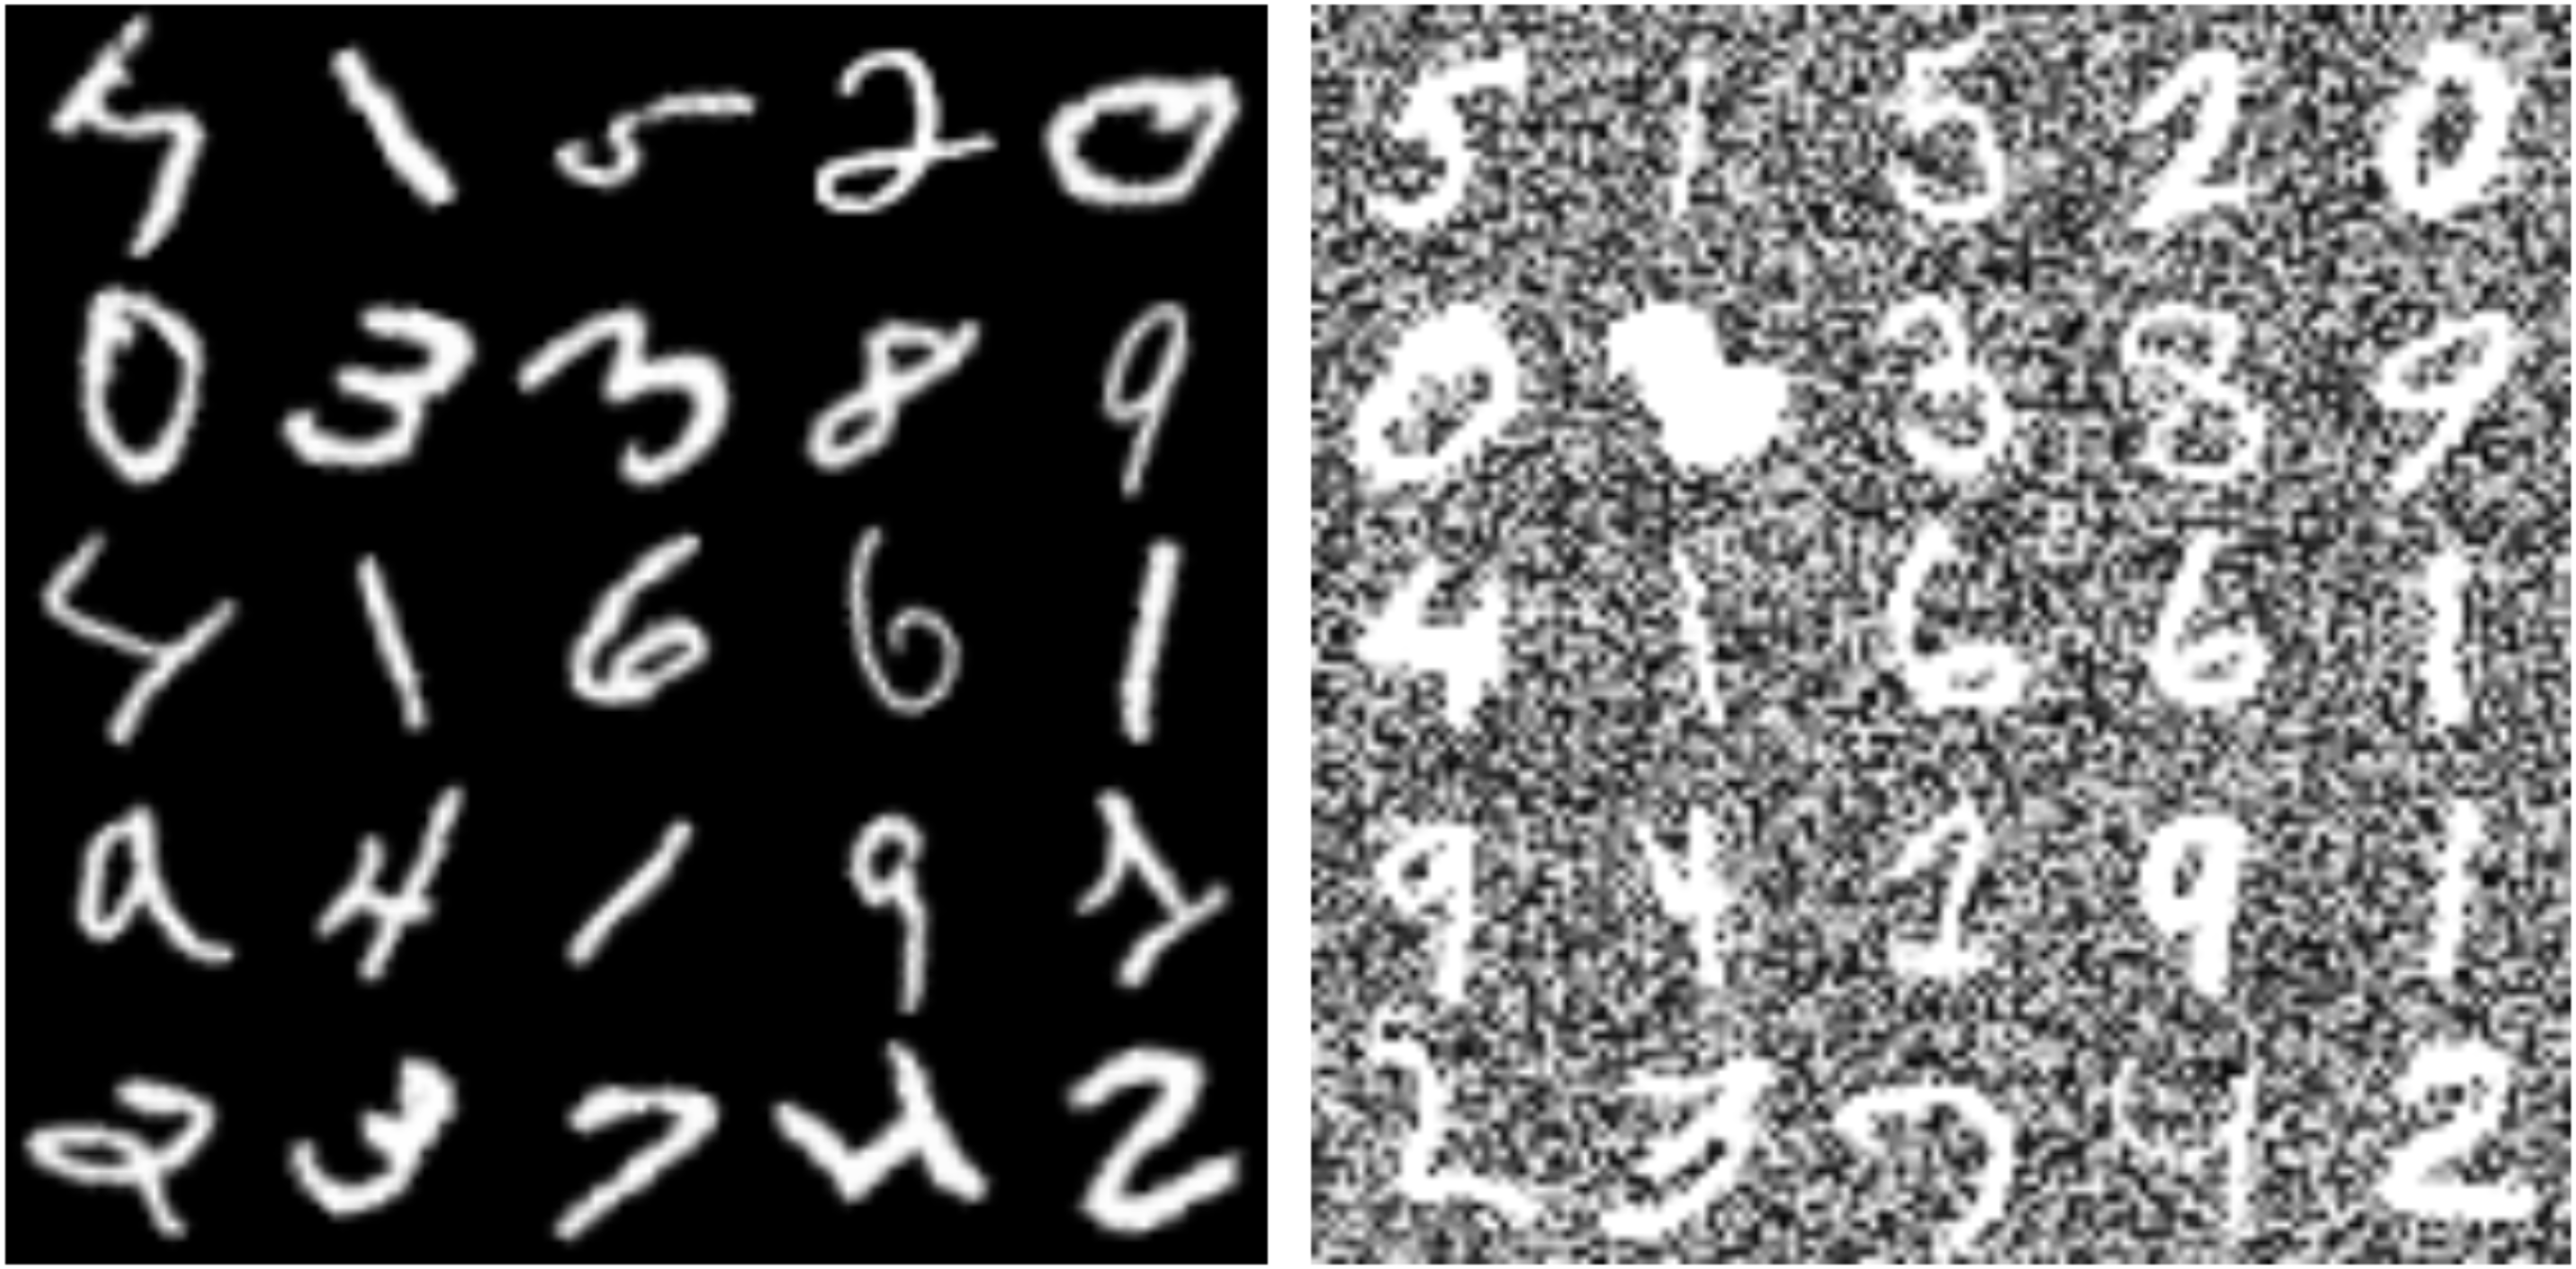
\includegraphics[width=\linewidth]{figures/noisy_mnist}
		\end{center}
		\caption{Зашумленные изображений из набора данных MNIST}
		\label{fgr:1}
	\end{figure}
	
	\begin{table}[h!]
		\caption{Точность классификации линейного SVM для алгоритмов Deep CCA и CCA.}
		\centering
		\begin{tabular}{l|cc}
			\hline
			Скользящий контроль & DeepCCA(L=3) & CCA \\  \hline
			Валидация & $92.74\%$  &  $76.21\%$\\
			Тест & $92.14\%$ & $76.07\%$ \\
			\hline
		\end{tabular}
		\label{tbl:1}
	\end{table}
	
	\section{Вычислительный эксперимент}
	Целью вычислительного эксперимента является анализ рассматриваемых моделей.
	Рассматриваются данные, для которых линейные методов являются слишком ограниченым классом моделей.
	Нелинейные модели позволяют получить точный прогноз при адекватной сложности.
	В рамках вычислительного эксперимента был написан программный комплекс для решения поставленных задач~\cite{source_code}.
	
	\subsection{Анализ нелинейных зависимостей в задаче устранения шума}
	
	Проведем сравнение качества Deep CCA и CCA на задаче классификации зашумленных цифровых изображений Рис.~\ref{fgr:1}. Для этого используется набор данных MNIST~\cite{MNIST}, который состоит из 70000 цифровых изображений $28 \times 28$ образцов рукописного написания цифр. Предлагается получить два новых набора данных $\bX$ и $\bY$ следующим образом. Первый набор получим поворотом исходных изображений на угол в диапазоне $[\frac{-\pi}{4}, \frac{\pi}{4}]$. Для получения второго набора данных для каждой картинки из первого набора данных ставится в соответствие случайным образом картинка с той же цифрой, но с добавлением независимого случайного шума, распределенного равномерно на отрезке $[0,1]$.
	
	Применив к двум новым наборам данных DeepCCA или CCA, мы получаем новое низкоразмерное признаковое пространство, которое игнорирует шумы в исходных данных. Таким образом, получаем функции кодирования $\varphi_1$ и $\psi_1$ для исходных наборов данных. На новых признаках, полученных разными моделями (DeepCCA и CCA), для первого набора данных, то есть на данных после применения функции кодирования $\varphi_1$ к первому набору исходных данных, обучим линейный SVM классификатор. Показателем эффективности будет точность классификации линейного SVM на тестовых данных. В случае построения адекватного скрытого пространства полученные образы объектов будут линейно разделимы. Результаты эксперимента приведены в Таблице~\ref{tbl:1}. Модель Deep CCA представляет из себя нейронную сеть с $L=3$ скрытыми слоями. Точность классификации нелинейной модели существенно выше линейного алгоритма CCA.
	
	
	\begin{figure}[h!]
		\begin{center}
			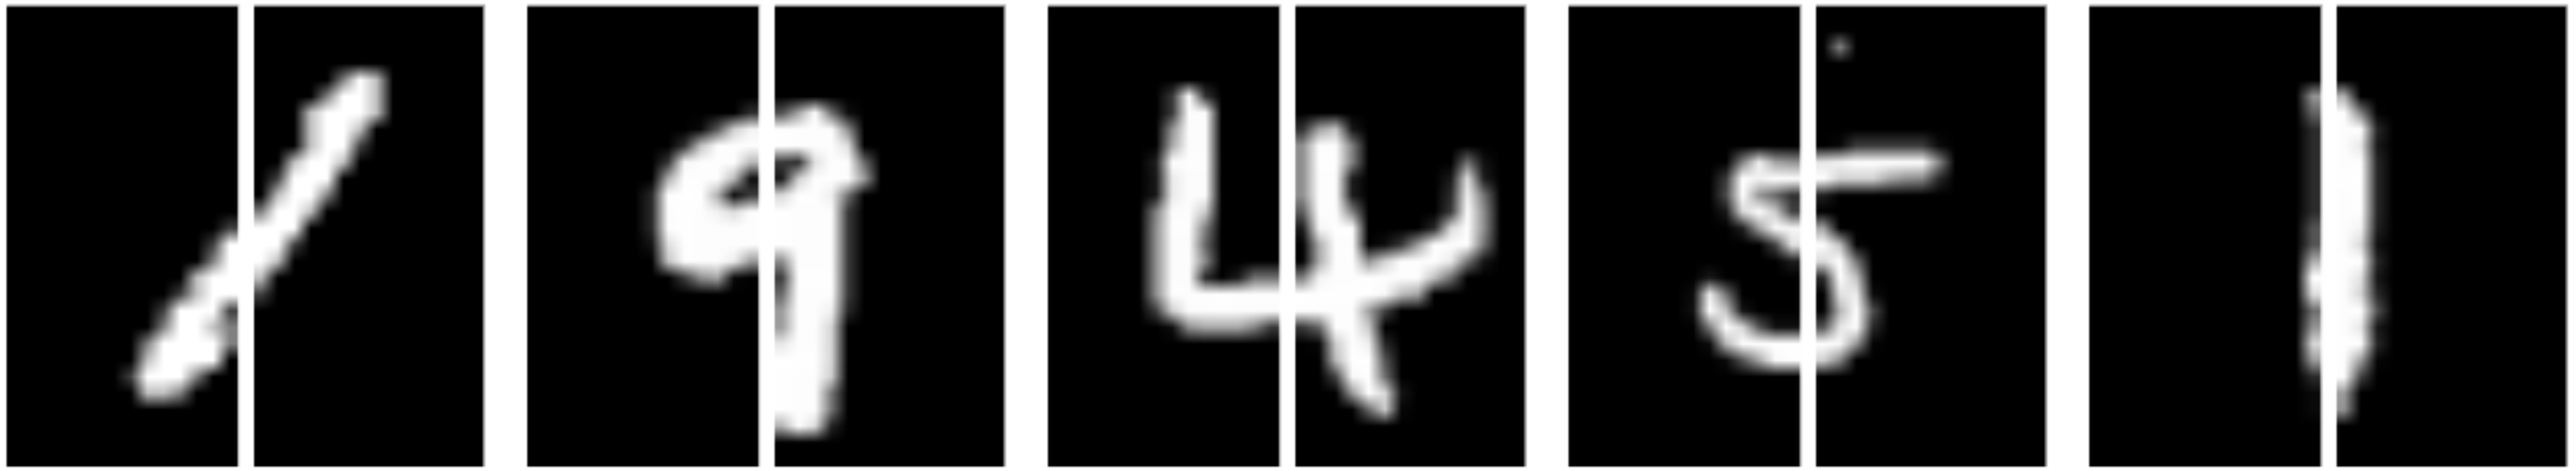
\includegraphics[width=\linewidth]{figures/left_right_mnist}
		\end{center}
		\caption{Набор данных MNIST, каждое изображение в котором разделили пополам.}
		\label{fgr:3}
	\end{figure}
	
	
	\begin{table}[h!]
		\caption{Восстановление правой части изображения по левой с использованием различных моделей. Для измерения качества моделей считается среднеквадратическое отклонения от оригинального изображения.
		}
		\centering
		\begin{tabular}{l|cccccc}
			\hline
			& EncNet1 & LinNet1 & EncNet2 & LinNet2 & DumbNet & PLS\\  \hline
			Кол-во весов & $283$k & $239$k & $283$k & $239$k  & $283$k & -\\ 
			MSE loss on test data & $0.147$ & $ 0.235$ & $0.149$ & $0.236$ & $0.128$ & $0.188$ \\ 
			\hline
		\end{tabular}
		\label{tbl:2}
	\end{table}
	
	\subsection{Анализ нелинейных моделей для восстановления изображений}
	
	Проведем на задаче регрессии сравнение нескольких моделей, которые используют автоэнкодеры для снижения размерности пространства, моделей без преобразования исходных данных и линейный PLS. Для этого используется набор данных MNIST. Каждое изображение делится на левую и правую части, как показано на Рис.~\ref{fgr:3}. Модель по левому изображению пытается посстановить правое изображение.
	
	Модель EncNet1~--- нейронная сеть с нелинейными функциями активации, которая обучается на данных после преобразования их автоэнкодером. Модель LinNet1~--- нейронная сеть с одним линейным слоем, которая также обучается на преобразованных данных. Для EncNet1 и LinNet1 автоэнкодеры для объектов и ответов используют совместную функцию потерь, которая связывает выходы енкодеров. Модели EncNet2 и LinNet2 устроены аналогично EncNet1 и LinNet1 соответственно, но в автоэнкодерах нет совместной функции потерь. Модель DumbNet~---  нейронная сеть, которая обучается на исходных данных и имеет такую же структуру, что и EncNet, то есть имеет такое же количество слоев и в каждом слое такое же количество нейронном, что и у EncNet.
	
	Для измерения качества моделей считается среднеквадратичная ошибка. Результаты работы алгоритмов показаны на изображении Рис.~\ref{fgr:2}. Качество работы моделей, а также их сложность представлены в Таблице~\ref{tbl:2}. 
	На Рис.~\ref{fgr:2} продемонстировано, что предложенные модели EncNet и LinNet позволяют получить более четкие и различимые изображения в отличие от базовой нелинейной модели DumbNet и линейной модели PLS.
	Несмотря на заметное улучшение визуального качества изображений, ошибка предложенных моделей выше, чем у модели DumbNet. 
	Авторы ставят гипотезу, что это связано с тем, что среднеквадратичная ошибка является неадекватной метрикой в пространстве изображений.
	Нахождение оптимальной метрики для оценки качества предложенных алгоритмов является одним из возможных направлений развития текущей работы.
	
	\begin{figure}[h!]
		\begin{center}
			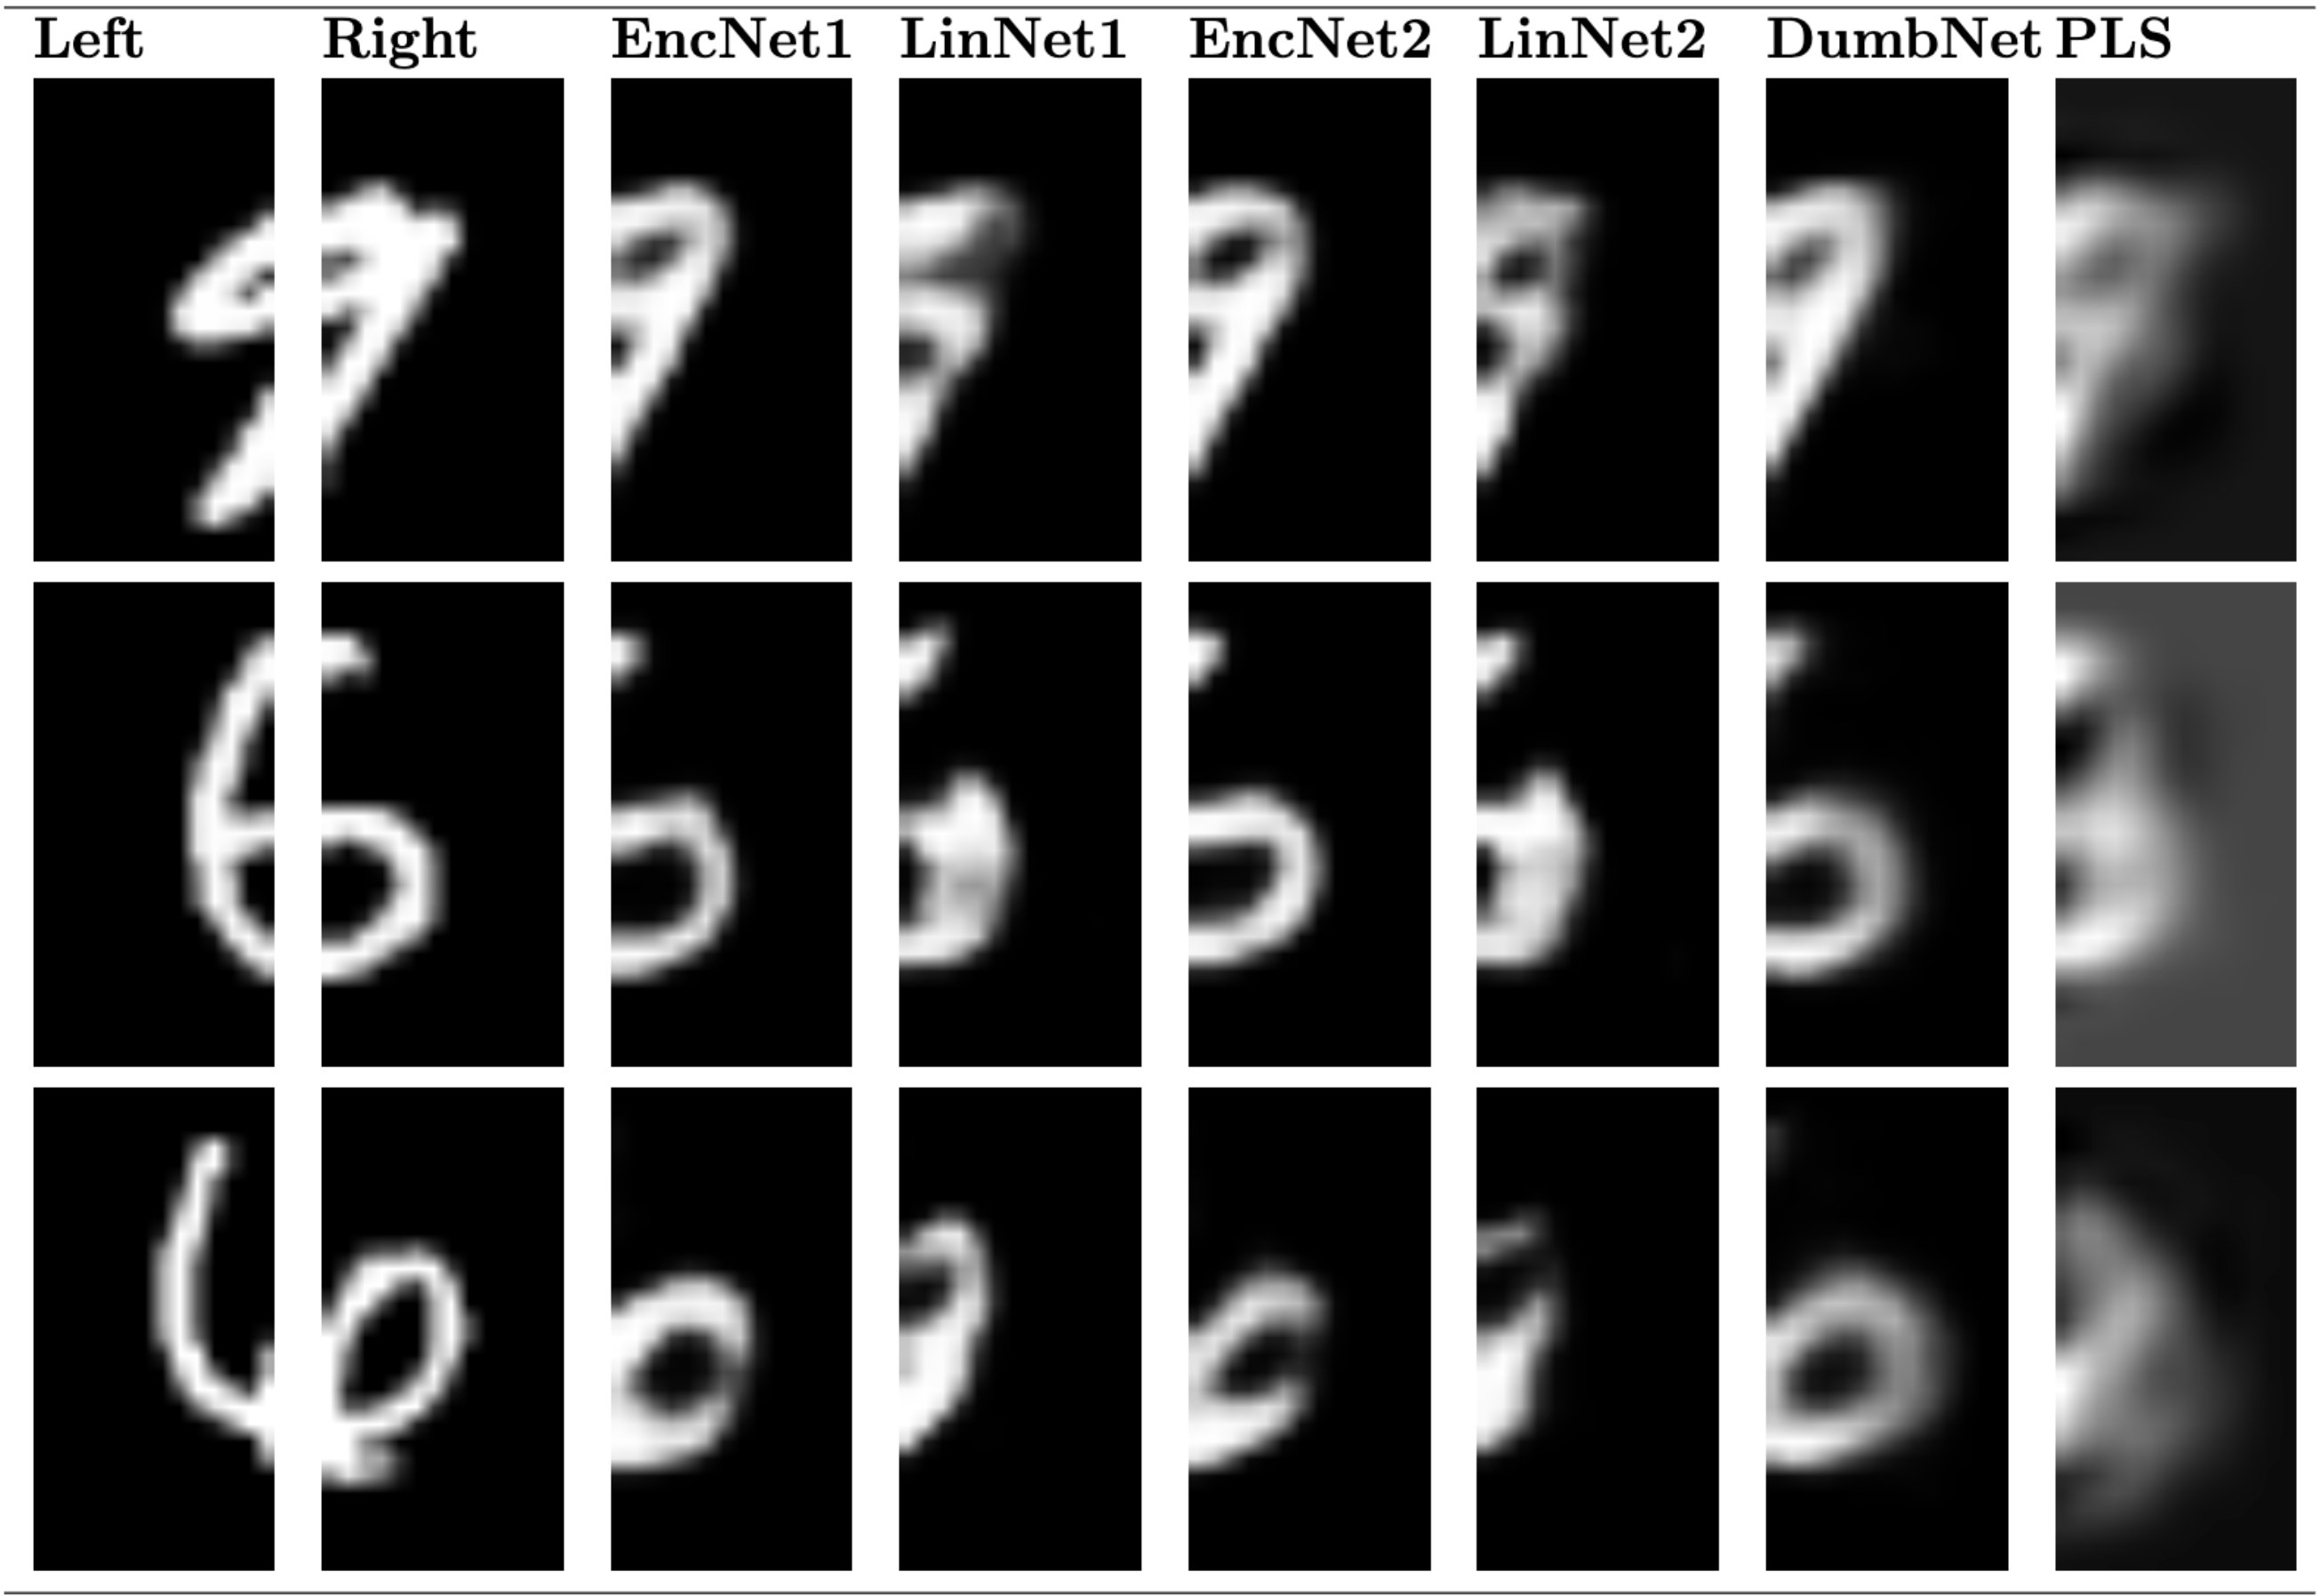
\includegraphics[width=\linewidth]{figures/mnist_preds}
		\end{center}
		\caption{Восстановление правой части изображения по левой.}
		\label{fgr:2}
	\end{figure}

	\section{Заключение}
	В работе рассмотрена задача декодирования для сложно организованной целевой переменной.
	Рассмотрены линейные модели согласования образов объектов в скрытом пространстве.
	В случае наличия сложных нелинейных зависимостей между независимой и целевой переменной сложности линейной модели оказывается недостаточно.
	Для построения точного прогноза приводятся нелинейные обобщения рассматриваемых линейных методов.
	В экспериментах на реальных данных изображений рукописных цифр показана адекватность рассматриваемых нелинейных моделей, а также проведен анализ различных способ согласования.
	
	\bibliographystyle{unsrt}
	\begin{thebibliography}{99}
		
		\bibitem{overview_pls}
		\textit{Rosipal R., Kramer N., Graves A.} Overview and recent advances in partial least squares~// International Statistical and Optimization Perspectives Workshop <<Subspace, Latent Structure and Feature Selection>>, 2005. P. 34--51.
		
		\bibitem{overview_nonlinear_pls}
		\textit{Rosipal R.} Nonlinear partial least squares: An overview~// Chemoinformatics and Advanced Machine Learning Perspectives, 2011. P. 169--189.
		
		\bibitem{1figures}
		\textit{Nguyen D. V., Rocke D. M.} Tumor classification by partial least squares using microarray gene expression data~// Bioinformatics, 2012.  Vol.~18. P.~39--50. 
		
		\bibitem{btc519}
		\textit{Worsley K. J.} An overview and some new developments in the statistical analysis of pet and fmri data~// Human Brain Mapping, 1997. Vol.~5. P.~254--258.
		
		\bibitem{PLS_in_strategic_management}
		\textit{Hulland J. S.} Use of partial least squares (pls) in strategic management research: A review of four recent studies~// Strategic Management Journal, 1999. Vol.~20. P.~195--204.
		
		\bibitem{PLS_application}
		\textit{Shalamu Abudu P. E., Pagano T. C.} Application of partial least-squares regression in seasonalstreamflow forecasting~// Journal of Hydrologic Engineering, 2010. Vol.~15. P.~612--623.
		
		\bibitem{cca_alg}
		\textit{Szedmak S. R., Hardoon D. R., Shawe-taylor J. R.} Canonical correlation analysis: An overview with application to learning methods.~// Neural computation, 2004. Vol.~16. P.~2639--2664.
		
		\bibitem{cca_apl1}
		\textit{Schechner Y. Y., Kidron E. Elad M.} Pixels that sound~// IEEE Computer Society, 2005. P.~88--95.
		
		\bibitem{cca_apl2}
		\textit{Sun S. Ji L., Ye J.} A least squares formulation for canonical correlation analysis~// International Confenence on Machine Learning, 2008. P.~1024--1031.
		
		\bibitem{PLS_nn}
		\textit{Qin S. J., McAvoy T. J.} Nonlinear pls modeling using neural networks~// Computers Chemical Engineering, 1992. Vol.~16. P.~379--391.
		
		\bibitem{PLS_rbf}
		\textit{Chen D. Z., Yan X. F., Hu S. X.} Chaos-genetic algorithms for optimizing the operating conditions based on rbf-pls model~// Computers and Chemical Engineering, 2003. Vol.~27. P.~1393--1404.
		
		\bibitem{PLS_ga}
		\textit{Hiden M., McKay B., Montague G.} Non-linear partial least squares using genetic programming~// Genetic Programming, 1998. P.~128--133.
		
		\bibitem{deep_cca}
		\textit{Chen D. Z., Yan X. F., Hu S. X.} Deep canonical correlation analysis~// International Confenence on Machine Learning, 2013. P.~1247--1255.
		
		\bibitem{kernel_cca}
		\textit{Lai P. L., Fyfe C.} Kernel and nonlinear canonical correlation analysis~// International Journal of Neural Systems, 2000. Vol.~10. P.~365--377.
		
		\bibitem{kernel_cca_appl}
		\textit{Yan F., Mikolajczyk K.} Deep correlation for matching images and text~// Computer Vision and Pattern Recognition, 2015. Vol.~4. P.~3441--3450.
		
		\bibitem{MNIST}
		\textit{LeCun Y.,  Cortes C., Burges C.} The MNIST dataset of handwritten digits, 1998. Available at: \url{http://yann.lecun.com/exdb/mnist/index.html}.
		
		\bibitem{source_code}
		\textit{Yaushev F. Yu,  Isachenko R. V.} Исходной код проекта доступен по ссылке:~\url{https://github.com/Fyaushev/2020-Project-72}, 2020.
	\end{thebibliography}
	
\end{document}

